\section{基于梯度的设计}\label{sec:gradient}

前面各节的工作点都由随机搜索得到。仿真器是可微分的（第~\ref{sec:lle}~节），所以也可以把器件参数和掩模当作可训练的量，
沿测试误差的梯度直接优化。可微分的 LLE 已被用来反向设计光梳的频谱形状~\cite{chuchalin2026}；这里的目标换成计算任务的误差，并把噪声放进优化里。
本节检验这样做能否胜过随机搜索。结论是：梯度微调能稳定地改善起点，但结果与扩大后的随机搜索打平，而后者用的计算少得多，
所以在本文的问题上，它不能代替随机搜索，最多是搜索之后的一步精修。

\subsection{训练设置}

可训练的量是失谐、输入耦合 $\Qone$、泵浦功率、调制深度和 16 根输入梳齿的复偏置与复权重（式~\eqref{eq:mask}）；
总输入光功率被限制在随机搜索的上限以内。
每次迭代把训练序列上的几个窗口（各 400 个符号，前面另有 100 个不求梯度的预热符号）各用几组独立的噪声实现同时跑一遍；
岭回归读出层在窗口的前一部分上闭式拟合（汇总所有窗口和噪声实现），在其余部分上计算 NMSE，
再加一项一致性惩罚（同一输入、不同噪声实现下标准化特征的方差，在混沌区接近 1）。
梯度穿过岭回归、读出和整个 LLE 积分传回器件参数。
训练中打开与现实噪声相同的各项噪声，而且读出层要同时拟合多组噪声实现，所以优化的是对噪声的期望误差，读出层也不能靠记住某一次实现取胜。

混沌区附近的损失面有陡崖：参数稍一越界，梳就进入不可重复的状态，梯度随之发散。我们用了四个保护措施：
梯度只回传 16 个符号（截断的随时间反向传播）；梯度裁剪；一步之后若损失远高于滑动平均就撤销这一步并把学习率减半；学习率按余弦衰减。
保留的参数是在另一条验证序列上得分最好的那一组，报告的误差来自第三条测试序列。

\subsection{网格截断陷阱}

训练用 256 个模式的谱网格以节省显存，报告前再在 512 个模式上重新仿真。
早期的训练用 128 个模式，这对本文的器件太窄：训练会把器件推向光谱更宽的工作点，让梳齿铺满整个网格。
一个例子是在 128 个模式上训练的环（无噪声、Mackey--Glass），训练后所有 128 个模式上都有可观的功率，
在 256 个模式、时间步减半的网格上复核时，光谱展宽到 215 根梳齿，测试误差从 $8.5\times10^{-3}$ 变为 $9.6\times10^{-3}$，相差约 14\%，
超过了本文其他结果里网格带来的差别（第~\ref{sec:lle}~节）。
网格边缘的截断成了优化器可以利用的一个“自由度”，得到的器件性能有一部分是离散化的产物。
所以可微分的物理模型做设计时，网格必须宽到截断不影响结果，而且每个训练结果都要在更细的网格上复核；本文图~\ref{fig:gradient} 的结果都在 512 个模式上复核过。

\subsection{与随机搜索的比较}

为了公平比较，我们从同一批随机工作点出发（现实噪声、8 个抽头的读出、Mackey--Glass，3 条序列）：
先抽 32 个随机点，按第一条序列的验证误差排序；取最好的 4 个点各用 2 个训练种子微调，再从排序中间取 4 个点各微调一次，共 12 次，每次 60 步。
作为对照，随机搜索从 32 个点扩大到 256 个点。所有结果都在 512 个模式上、用新的噪声实现复测（图~\ref{fig:gradient}）。

\begin{figure}[htbp]
\centering
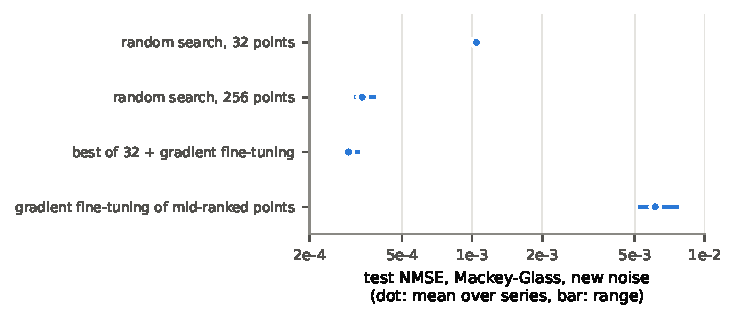
\includegraphics[width=0.75\linewidth]{fig7_gradient}
\caption{梯度微调与随机搜索的比较（现实噪声下的 Mackey--Glass，512 个模式、新噪声复测；点为 3 条序列的平均，横线为范围）。
从 32 个随机点中最好的点出发微调，与把随机搜索扩到 256 个点的结果相当；从排序中间的点出发，微调后仍远差于搜索。}
\label{fig:gradient}
\end{figure}

12 次微调全部好于各自的起点，误差降到起点的 0.24 到 0.93 倍，几何平均约 0.46 倍。
32 个随机点中最好的点为 $1.04\times10^{-3}$，从它出发微调后最好为 $2.9\times10^{-4}$；
而把随机搜索扩到 256 个点，直接得到 $3.4\times10^{-4}$，两者相当，差别在噪声实现之间的波动范围内。
另外三点限制了梯度微调的作用：
同一个起点换一个训练种子，结果相差近 2 倍（$2.9\times10^{-4}$ 对 $5.4\times10^{-4}$）；
从排序中间的点出发，微调后仍在 $6\times10^{-3}$ 以上，远差于搜索得到的点，也就是说微调救不了中等的起点；
12 次中有 3 次在最后一次验证（第 60 步）时仍是最好的，说明这几次还没有收敛，更长的训练可能还有收益。
计算量上随机搜索占明显优势：在同一块显卡上，每次微调（256 个模式、60 步）每步约 18 秒，一次约 18 分钟，从最好的 4 个起点出发的 8 次微调合计约 2.4 小时；
而把随机搜索从 32 个点扩到 256 个点，每条序列只多出一批批量仿真（一批最多 512 个工作点，约一到两分钟）。

所以在本文的参数规模下（约 70 个实数参数），单用随机搜索更划算；梯度微调最多适合作为搜索之后的精修，而且要换几个训练种子。
可微分仿真可能在两种情况下更有价值：一是可调的量很多（例如 64 根梳齿的掩模，或者多个环一起设计），随机搜索的效率会迅速下降，而梯度的代价几乎不变；
二是目标函数中有随机搜索难以覆盖的连续结构。这两点本文都没有检验。
